% !TEX root = mainthesis.tex
%Chapter 2

\renewcommand{\thechapter}{2}

\chapter{Basic theory of Bose-Einstein condensation}

Bose-Einstein condensation (BEC) is a quantum state of mater in which particles with integer valued spin all tend to occupy or `condense' into the ground state. In dilute gases, condensation occurs when the temperature of the system goes bellow a critical temperature where the bosons become indistinguishable particles and quantum statistics become relevant. 

BECs enable the observation of macroscopic quantum phenomena and there have been a number of fascinating experiments studying the properties of this systems, from measuring interference fringes of a macroscopic wave function to studying collective effects such as the propagation of sound~\cite{ketterle_w._making_1999}, as well as extensive theoretical developments~\cite{dalfovo_theory_1999}. In our experiments however BECs are not the primary object of study, instead they are used as a platform enabling the simulation of analogue physical systems. 

In this Chapter I give an overview of Bose-Einstein condensation in dilute atomic gases and I describe the properties most relevant to our experiments. I start by describing the case of an ideal gas and then consider the effects of interactions and trapping potentials as are present in our case. A reader interested in learning about this subject in more depth is advised to read~\cite{Pethick} and~\cite{noauthor_bose-einstein_2003}.

\section{Bose-Einstein condensation of an ideal gas}

At low temperatures and in thermodynamic equilibrium, the mean occupation number of non-interacting identical bosons in the state with energy $E$ is given by the Bose-Einstein distribution
%
\begin{equation}
	n(E_j)=\frac{1}{e^{(E_j-\mu)/k_BT}-1}
	\label{eq:Bose_distribution}	
\end{equation}
%
where $T$ is the temperature, $\mu$ is the chemical potential (the energy cost of adding or removing a particle) and $k_B$ is the Boltzmann constant. In the limit of large temperatures the Bose distribution can be approximated by the Maxwell-Boltzmann distribution
%
\begin{equation}
	n(E_j)\approx e^{-(E_j-\mu)/kT}
\end{equation}
%
which applies to classical, distinguishable particles. The chemical potential is determined by the condition that the total number of particles $N$ is equal to the sum over all states in the distribution $N=\sum_jn(E_j)$ and is therefore a function of $N$ and $T$. Additionally, in order for $n(E_j)$ to be positive definite we must have $\mu\leq E_0$ where $E_0$ is the energy of the ground state. From the Bose distribution we can see that the occupation number of the ground state is unbounded when $\mu\rightarrow0$ as is shown in Figure~\ref{eq:Bose_distribution}. The number of particles occupying the excited states is bounded and when that number is reached, the remaining particles can occupy the ground state and thus Bose-Einstein condensation occurs. 

\begin{figure}[htb]
\begin{center}
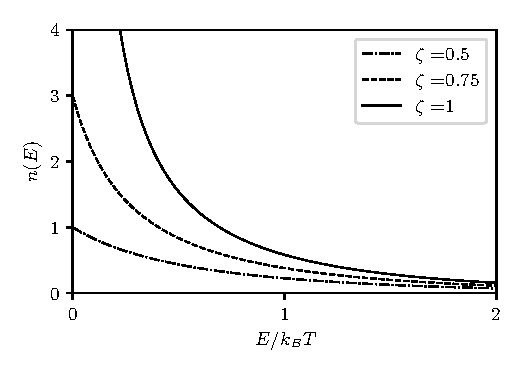
\includegraphics[]{Figures/Chapter2/Bose_distribution.pdf}
\caption[The Bose-Einstein distribution]{The Bose-Einstein distribution. Occupation number as a function of energy for different values of fugacity $\zeta=\exp(\mu /k_BT)$. Condensation occurs when $\mu=0$ ($\zeta=1$) and the occupation number in the ground state diverges.}
\label{fig:Bose_distribution}
\end{center}
\end{figure}

\subsection{Critical temperature}

Bose-Einstein condensation can be understood in terms of the de Broglie waves associated to particles. The thermal de Broglie wavelength is defined as
%
\begin{equation}
	\lambda_{\rm{th}}=\left(\frac{2\pi\hbar^2}{mk_BT}\right)^{1/2}
\end{equation}
%
and it characterized the spatial extension of the wave packet an individual particle at temperature $T$. Condensation occurs when $\lambda_{\rm{th}}$ becomes comparable with the inter-particle separation $n^{-1/3}$, where $n=N/V$. The quantity $n\lambda_{\rm{th}}^3$ is known as the phase space density which describes the number of particles contained in a box with volume $\lambda_{\rm{th}}^3$. 

An analytical expression for the critical temperature at which atoms condense can be derived using the Bose-Einstein distribution. For closely spaced energy levels (compared to $k_B T$) the sum representing the total number of particles can be replaced by the integral
%
\begin{equation}
	N=\int_0^\infty n(E) g(E) dE
	\label{eq:N(E)}
\end{equation}
%
where $g(E)$ is the density of states and $g(E)dE$ corresponds to the number of available states with energy between $E$ and $E+dE$. For a free particle in three dimensions the density of states is
%
\begin{equation}
	g(E)=\frac{V m^{3/2}}{\sqrt{2}\pi^2\hbar^2}E^{1/2},
	\label{eq:free_particle_dos}
\end{equation}
%
and in general the density of states can be expressed as a power of energy $g(E)=C_\alpha E^{\alpha-1}$. 

The integral in Equation~\ref{eq:N(E)} is not analytically solvable, however we can make the simplifying assumption $\mu=0$. The critical temperature $T_c$ is determined by the condition that all particles are in the excited states
%
\begin{align}
	N&=N_{\rm{ex}}(T_c, \mu=0) \nonumber \\
	&=\int_0^{\infty}\frac{g(E)dE}{e^{E/k_BT_c}-1} \nonumber \\
	&= C_\alpha(k_BT_c)^\alpha\int_0^\infty\frac{x^{\alpha-1}}{e^x-1} \nonumber \\
	&= c_\alpha (k_BT_c)^\alpha\Gamma(\alpha)\zeta(\alpha)
	\label{eq:finding_Tc}
\end{align}
%
where I made the substitution $x=E/k_BT_c$, $\Gamma(\alpha)=\int_0^\infty x^{\alpha-1}e^{-x}dx$ is the Gamma function and $\zeta(\alpha)=\sum_{n=1}^\infty n^{-\alpha}$ is the Riemann zeta function. From Equation~\ref{eq:finding_Tc} we find that the critical temperature for Bose-Einstein condensation is
%
\begin{equation}
	k_BT_c=\left(\frac{N}{C_\alpha\Gamma(\alpha)\zeta(\alpha)}\right)^{1/\alpha}.
\end{equation}

If we compute the phase space density for free particles in 3D with density of states  given by Equation~\ref{eq:free_particle_dos} in combination with the expression for the critical temperature (Equation~\ref{eq:finding_Tc} we find that indeed when $T=T_c$
%
\begin{equation}
	n\lambda_{\rm {th}}^3=\zeta\left(\frac{3}{2}\right)\approx 2.612,
\end{equation}
%
the inter particle spacing and the thermal wavelength are comparable. In order to experimentally produce BECs, a combination of laser and evaporative cooling techniques are deployed such that we can increase the density while minimizing the temperature and therefore maximize the phase space density. The densities for BECs of Alkali atoms typically range in of order $10^{13}$ to $10^{15}$ atoms/cm$^{-3}$.

\subsection{Condensate fraction}

Now we look at the fraction of particles occupying the ground state at temperatures below $T_c$. The total number of particles is given by $N=N_0+N_{\rm{ex}}$. The number of particles in the excited state will be given by the integral in Equation~\ref{eq:N(E)}. For $g(E)=C_\alpha E^{\alpha-1}$and $\alpha>0$ the integral converges, we can then evaluate the integral in Equation~\ref{eq:finding_Tc} for $T<T_c$ and get
%
\begin{align}
	N_{\rm{ex}}&=c_\alpha (k_BT)^\alpha\Gamma(\alpha)\zeta(\alpha) \nonumber \\
	&=N\left(\frac{T}{T_c}\right)^\alpha,
\end{align}
%
where I used the fact that when $T=T_c$ the total number $N=N_{\rm{ex}}$. The number of particles in the ground state is therefore
%
\begin{align}
	N_0&=N-N_{\rm{ex}} \nonumber \\
	&= N\left[1-\left(\frac{T}{T_c}\right)^\alpha\right]
\end{align}

\subsection{Bose gas in a harmonic trapping potential}

I consider the particular case of particles confined in a three dimensional harmonic potential
%
\begin{equation}
V(\r)=\frac{m}{2}\left(\omega_x^2x^2+\omega_y^2y^2+\omega_z^2z^2\right)
\label{eq:ho}
\end{equation}
%
as it is the most relevant to our experiments that are performed in optical dipole traps that can be described as harmonic potentials. The density of states for is 

\begin{equation}
	g(E)=\frac{E^2}{2\hbar^2\omega_x\omega_y\omega_z},
\end{equation}
%
which corresponds to $\alpha=3$ and $C_3=(2\hbar^3\omega_x\omega_y\omega_z)^{-1}$. Using Equation~\ref{eq:finding_Tc}, we find that the transition temperature is
%
\begin{equation}
 	k_B T_c=\frac{\hbar \bar{\omega}N^{1/3}}{\zeta(3)^{1/3}}\approx0.94\hbar\bar{\omega}N^{1/3}
 \end{equation} 
%
where $\bar{\omega}=(\omega_x\omega_y\omega_z)^{1/3}$ is the geometric mean of the oscillation frequencies. Similarly we find that the condensed fraction is
%
\begin{equation}
	N_0=N\left[1-\left(\frac{T}{T_c}\right)^3\right]
\end{equation}

Condensates in harmonic traps have some striking features that will be further explored in more detail in the following sections. The confining potential makes the BECs both finite sized and inhomogeneous which means that the BEC can be observed both in momentum space and in coordinate space. Another consequence of the inhomogeneity of these systems is the role of two-body interactions, which gets enhanced and leads to noticeable effects in measurable quantities~\cite{dalfovo_theory_1999,castin_bose-einstein_1996} such as interaction driven expansion when they are released from the confining potential. Some of these features will be discussed in more detail in the following sections.

\section{Bose-Einstein condensation with atomic interactions}

Even though atomic BECs are made from very dilute gases, the system is far from being an ideal gas and interactions need to be taken into account for a complete treatment.% of the system. 

The collisional properties of particles at low energies, such as cold atoms in a condensate, are dominated by $s$-wave scattering which can be described in terms of a single parameter the scattering length $a$ that determines both the scattering cross section $\sigma=4\pi a^2$ and the phase shift of the scattered wave function. 

The magnitude of the scattering length is determined by the interatomic interaction potentials. For Alkali atoms at large distances, the two-body interactions are dominated by an attractive Van der walls interaction $U(r)=-C_6/r^6$ that arises from dipole-dipole interactions. At smaller distances the attractive potential is replaced by a strong repulsive electron-exchange interaction $U(r)\rightarrow\infty$. This minimal model captures the most important properties of the inter-atomic potential and can be solved analytically~\cite{gribakin_calculation_1993}. 

If the range of the interaction is much shorter than the mean inter-atomic distance the interaction can be approximated by an effective pseudo-potential $U_{\rm{eff}}(\r-\r')$ such that
%
\begin{equation}
	a=\frac{m}{4\pi\hbar^2}\int U_{\rm{eff}}(\r-\r')d \r
\end{equation}
%
which determines
%
\begin{equation}
	U_{\rm{eff}}(\r-\r')=\frac{4\pi\hbar^2a}{m}\delta(\r-\r')=g\delta(\r-\r').
\end{equation}
%
This is a nice approximation as it allows us to model the scattering between atoms as a hard sphere scattering process instead of considering the more complicated inter-atomic potentials. The sign of the scattering length determines the attractive or repulsive nature of the interactions and it  plays an important role in the experimental production of BECs as it determines the rate at which atoms thermalize during evaporative cooling. 

\subsection{Gross-Pitaevskii equation}

The full Hamiltonian describing $N$ identical bosons with contact interactions can be written as
%
\begin{equation}
	\hat{H}=\sum_{i=1}^N\left[\frac{\mathbf{p}_i^2}{2m}+V(\r_i)\right]+g\sum_{i<j}\delta(\r_i-\r_j),
	\label{eq:many_body_h}
\end{equation}
%
where $V(\r)$ is an external potential and $\mathbf{p}_i=-i\hbar\nabla_i$ is the momentum. We now consider a normalized eigenstate of the Hamiltonian $\Psi(\r_1, \r_2, ..., \r_N)$ that satisfies the Schr\"odinger equation. We can simplify this state by taking a mean field approach; we assume that the system has undergone condensation so that the majority of the particles share the same single particle ground state $\phi(\r)$ the wavefunction can be approximated by a symmetrized product
%
\begin{equation}
	\Psi(\r_1, \r_2, ..., \r_N)=\prod_{i=1}^N\phi(\r_i),
	\label{eq:mean_field_psi}
\end{equation}
%
where $\phi$ is normalized to unity. The energy of the state from Equation~\ref{eq:mean_field_psi} is given by the expectation value
%
\begin{align}
	E&=\int\Psi^*\hat{H}\Psi \,d\r \nonumber \\
	&=N\int\phi^*(\r)\left[-\frac{\hbar^2}{2m}\nabla^2+V(\r)+\frac{(N-1)}{2}g\vert \phi(\r)\vert^2\right]\phi(\r) d\r,
	\label{eq:mean_field_E}
\end{align}
%
where $N(N-1)/2\approx N^2/2$ counts the number of terms in the interaction energy. Now we introduce the wave function of the condensate $\psi(\r)=N^{1/2}\phi(\r)$, which when inserted in Equation~\ref{eq:mean_field_E} makes the $N$ factors cancel out. The optimal form of $\psi$ should minimize the energy subject to the normalization condition $N=\int\vert\psi(\r)\vert^2\,d\r$. This can be done by introducing a Lagrange multiplier $\mu$ so that
%
\begin{align}
	\frac{\delta}{\delta \psi^*(\r)}\left(E-\mu\int\vert\psi\vert^2\,d\r \right) 
	&= \left[-\frac{\hbar^2}{2m}\nabla^2+V(\r)+g\vert\psi(\r)\vert^2-\mu\right]\psi(\r)
	=0,
\end{align}
%
and we thus find that the condensate wave function obeys a non-linear Schr\"odinger equation known as the Gross-Pitaevskii (GP) equation.
%\footnote{The GP equation is very minimally relevant to my experiment but it still feels good knowing where it comes from.}.  
%
\begin{equation}
	\left[-\frac{\hbar^2}{2m}\nabla^2+V(\r)+g\vert\psi(\r)\vert^2\right]\psi(\r)=\mu\psi(\r)
\end{equation}
%
where $\mu$ plays the role of the chemical potential. The dynamics of the condensate will similarly be described by the time-dependent GP equation
%
\begin{equation}
	i\hbar\frac{\partial}{\partial t}\psi(\r,t)=\left[-\frac{\hbar^2}{2m}+V(\r)+g\vert\psi(\r,t)\vert^2\right]\psi(\r,t)
\end{equation}

The GP equation is useful for describing the relevant phenomena associated with BECs, for example the propagation of collective excitations and the expansion of the condensate when released from a trap. The crucial assumption when deriving these equations was the mean field approximation which should be valid for dilute BECs in which the condensate fraction is close to unity. The excitations of the system can be described by a set of equations similar to those of classical hydrodynamics derived from the GP equation or alternatively using Bogoliubov theory for weakly interacting bosons\cite{Pethick}.

\subsection{Multiple component BECs}

So far the discussion has been limited to single component BECs but most of our experiments are performed using a combination of multiple atomic internal states. In general, for a multiple component condensate the scattering lengths characterizing the interactions depend on the internal states of the incoming and outcoming scattering channels. Two spin-$f$\footnote{Here I use the simbol $f$ to denote the angular momentum of the individual particles and $F$ to denote the total angular momentum of the two particles.} particles colliding particles will be characterized by $2f$ scattering lengths $a_F$. For bosons the total spin $F$ takes even values and in particular for $\Rb87$ atoms in the $f=1$ hyperfine ground state there are two scattering lengths $a_0$ and $a_2$ corresponding to the two-particle total angular momentum states of $F=0$ and $F=2$ respectively. The values of scattering lengths are $a_0=101.8a_0$ and $a_2=100.4a_0$~\cite{stamper-kurn_spinor_2013} where $a_0=5.29\times 10^{-11}$ is the Bohr radius. From the scattering lengths we can calculate two interaction coefficients
%
\begin{align}
	c_0&=\frac{4\pi\hbar^2}{m}\frac{a_0+2a_2}{3}=100.84a_0\frac{4\pi\hbar^2}{m} \nonumber \\
	c_2&=\frac{4\pi\hbar^2}{m}\frac{a_0-a_2}{3}\approx -4.7\times 10^{-3}c_0.
\end{align}
%
Here $c_0$ represents a spin-independent interaction strength that depends only on the total density while $c_2$ is a spin-dependent energy that is relevant only where there is non-zero density of both atoms in $m_F=\pm1$ and is much smaller than the spin-independent energy. Similar to the case of single component BECs, the dynamics of multiple component BECs is governed by a spinor GP equation (see\cite{Pethick,stamper-kurn_spinor_2013}). The spin-dependent interaction strength gives rise to processes like coherent spin-mixing oscillations and domain formation and coarsening which was previously studied in the our lab~\cite{de_quenched_2014}.

The time scale at which interactions become relevant is set by the interaction energies $n \vert c_i\vert$. The most noticeable effect of interactions in our system is the density profile of the condensate and its anisotropic expansion after it is released from a trap which I will describe in the following sections. For the typical densities and timescales of our experiments as well as the relatively high magnetic fields that we operate at, we do not observe noticeable effects from interactions in the dynamics of the system and in the remaining chapters I will describe the dynamics of the BEC using single particle physics (i.e. the regular time-dependent Schr\"odinger equation). 

% Relationship between spin-dependent energy $n\vert c_2\vert$ and quadratic Zeeman shift gives time scale for spin-dependent interaction driven dynamics and is not very relevant for our experiments. 

% What should be taken away from these sections is that interactions matter and are necessary for the full description of a BEC of dilute gases, however for usual densities and interaction strengths in our $\Rb87$ BECs as well as the time scales of our experiments interactions play a very minimal role in the dynamics of the system and in fact they will be completely ignored in the remaining chapters. 

% For  $\Rb87$ at zero magnetic field $a=103 a_0$\cite{stamper-kurn_spinor_2013} where $a_0=\unit[5.29\times10^{-11}]{m}$ is the Bohr radius while for the more abundant isotope $^85$Rb $a=-\unit[23.44]{nm}$ which means that a BEC with density beyond a critical value can collapse~\cite{gerton_direct_2000}. \note{TODO: try to find references for the values of scattering lengths}

\subsection{Thomas-Fermi approximation}
\label{sec:Thomas-Fermi}

For systems with large $N$, the interaction term in the GP equation is very large compared to the kinetic energy\footnote{It can be shown that the ratio of kinetic energy to interactions scales like $N^{-4/5}$}. As the kinetic energy becomes less important we enter the Thomas-Fermi (TF) regime where the energy of the system is given only by the external potential and the mean field energy and the GP equation is considerably simplified 
%
\begin{equation}
	\left[V(\r)+g\vert\psi(\r)\vert\psi(\r)\vert^2\right]\psi(\r)=\mu\psi(\r).
\end{equation}
%

In the TF regime the density distribution of the condensate $n(\r)=\vert\psi(\r)\vert^2$ reflects the shape of the external potential
%
\begin{equation}
	n(\r)=g^{-1}[\mu-V(\r)],
\end{equation}
%
when $\mu-V(\r)>0$ and is otherwise zero. For a harmonic confining potential (Equation~\ref{eq:ho}) as is typical in our experiments we find that the length scale that characterizes the size of the condensate is the Thomas-Fermi radius
%
\begin{equation}
	R_j=\sqrt{\frac{2\mu}{m\omega_j^2}}, \ \ \ j=x,y,z.
\end{equation}
%
The density of the condensate is described by an inverted parabola
%
\begin{equation}
	n(\r)=\frac{\mu}{g}\left(1-\frac{x^2}{R_x^2}-\frac{y^2}{R_y^2}-\frac{z^2}{R_z^2}\right).
	\label{eq:n_tf}
\end{equation}
 %
as is shown in Figure~\ref{fig:Thomas_fermi}a. By integrating over Equation~\ref{eq:n_tf} we find that
 %
 \begin{equation}
 	N=\frac{8\pi}{15}\frac{\mu}{g}R_xR_yR_z,
 	\label{eq:condensate_number}
 \end{equation}
 %
 which allows to determine the number of atoms in the condensate based on the density profile. In practice, in-situ BECs are very dense which can lead to some technical difficulties when trying to image directly their density profiles (see Section~\ref{sec:absorption imaging}) so instead our images are taken after the atoms are released from the trap and allowed to expand for some time. In the next section I will discuss how the density profiles of atomic clouds are modified after they are released from a confining potential. 

\begin{figure}[htb]
\begin{center}
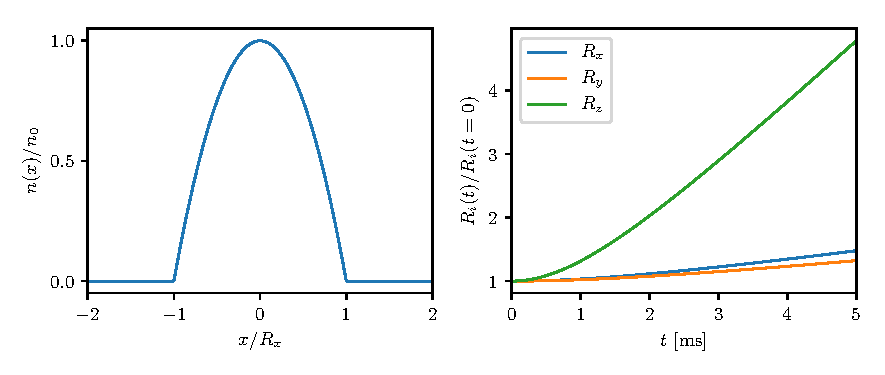
\includegraphics[]{Figures/Chapter2/Thomas_fermi.pdf}
\caption[The Thomas-Fermi density distribution]{In the Thomas-Fermi regime where interactions are large compared to kinetic energy the density profile is determined by the external potential.{\bf a.}Density profile along $\ex$ of a BEC in a harmonic potential. {\bf b.} Interaction driven expansion of a BEC in time-of-flight for a trap with trapping frequencies $(\omega_x, \omega_y, \omega_z)=\unit[2\pi(42, 34, 133)]{Hz}$  obtained by numerically integrating Equation~\ref{eq:castin_dum_radius}.}
\label{fig:Thomas_fermi}
\end{center}
\end{figure}

\section{Density profiles}

Most ultracold atoms experiments are probed by directly imaging the atoms (e.g. with absorption imaging, Section~\ref{sec:absorption imaging}). If the atoms are imaged in-situ we gain access to their spatial density profiles. If the atoms are released from the trap and allowed to expand in time of flight (TOF) we gain access to their momentum distribution. In this section I summarize the signatures in the density distributions of BECs and thermal atoms confined in a harmonic potential both in-situ and after TOF. 

For the case of a BEC confined in a harmonic potential at zero temperature (no thermal fraction) and in the Thomas-Fermi regime discussed in Section~\ref{sec:Thomas-Fermi}, the in-situ density distribution is described by 
%
\begin{align}
	n(\r)&=n_0\left(1-\frac{x^2}{R_x^2}-\frac{y^2}{R_y^2}-\frac{z^2}{R_z^2}\right) \nonumber \\  
	&= \frac{15N}{8\pi R_xR_yR_z}\left(1-\frac{x^2}{R_x^2}-\frac{y^2}{R_y^2}-\frac{z^2}{R_z^2}\right).
	\label{eq:n_thomas-fermi}
\end{align}

Even though the BEC is in the motional ground state, it will expand during TOF as a consequence of interactions. The expansion can be determined using the time dependent GP equation. A detail account of the procedure can be found in \cite{castin_bose-einstein_1996}, the procedure relies on using the ansatz that the TF radii expand as
%
\begin{equation}
	R_i(t)=\lambda_i(t)R_i(t=0),
	\label{eq:castin_dum_radius}
\end{equation}
%
where I assumed that the condensate is in the trap at $t=0$ which implies that $\lambda_i(0)=1$. The trap is then suddenly turned off at $t>0$. If we insert the condensate wave function with TF radii given by Equation~\ref{eq:castin_dum_radius} into the time-dependent GP equation we find a series differential equations
%
\begin{equation}
	\frac{d^2\lambda_i}{dt^2}=\frac{\omega_i^2}{\lambda_i\lambda_x\lambda_y\lambda_z}
\end{equation}
%
which can be used to determine the density profile of the BEC in TOF. Alternatively if the density profile of the BEC is known from an image, these relations can used to back-propagate what the original TF radii of the confined condensate was. This is helpful for example to calculate the atom number in the condensate using Equation~\ref{eq:condensate_number}. Figure~\ref{fig:Thomas_fermi}b shows the scaling factors $\lambda_i$ as a function of TOF that were obtained by numerically integrating Equation~\ref{eq:castin_dum_radius} for for a harmonic potential with frequencies close to those characterizing the optical dipole trap used in the lab.

For a thermal gas in a harmonic potential at temperatures higher than the level spacing $k_BT>\hbar\omega_{x,y,z}$ the density is given by~\cite{ketterle_w._making_1999}
%
\begin{equation}
	n_{\rm{th}}(\r)=\frac{1}{\lambda_{\rm{th}}^3}g_{3/2}(z(\r))
\end{equation}
%
where $z(\r)=\exp(\mu-V(\r)/\k_BT$, $V(\r)$ is given by Equation~\ref{eq:ho}, $\mu$ is the chemical potential and $g_j(z)=\sum_iz^i/i^j$ is the Bose function. The Bose function introduces effects of quantum statistics and compared to the Maxwell-Boltzmann distribution of distinguishable particles, the peak density of a Bose gas is increased by $g_{3/2}(z)/z$, a phenomenon known as Bose-enhancement.

The distribution after TOF can be calculated considering that the trapped atoms fly ballistically from their position in the trap. An atom starting initially at the point $\r_0$ moves to the point $\r$ after a time $t$ if its momentum is given by $\mathbf{p}=m(\r-\r0)/t$, and it can be shown that
%
\begin{align}
	n_{\rm{tof}}&=\frac{1}{\lambda_{\rm{th}}}\prod_{i=1}^3g_{3/2}\left(\exp\left[\mu-\frac{m}{2}\sum_{i=1}^3x_i^2\left(\frac{\omega_i^2}{1+\omega_i^2t^2}\right)\right]\right) \nonumber \\
	&\approx \frac{1}{\lambda_{\rm{th}}}g_{3/2}\left(\exp\left[(\mu-\frac{mr^2}{2t^2})/k_BT\right]\right)
	\label{eq:n_thermal}
\end{align}
%
where the approximation in the second line is valid for $t\gg \omega_i^{-1}$. The temperature of the atoms can be estimated by looking at the wings of the density distribution after TOF. Even with the case of Bose enhancement, the density of the wings still decays exponentially as $\exp(-x_i^2/2\sigma_i^2)$. The temperature of the cloud can be determined using
%
\begin{align}
	k_BT&=\frac{m}{2}\left(\frac{\omega_i^2}{1+\omega_i^2t^2}\sigma_i^2\right) \nonumber \\
	&\approx \frac{m}{2}\left(\frac{\sigma_i}{t}\right)^2
\end{align}

For partially condensed clouds the density profiles will be given by a combination of the thermal density profiles and the Thomas-Fermi density profile. Figure~\ref{fig:BEC_transition} shows the density distributions of atoms extracted from images taken after a $\unit[21]{ms}$ TOF and therefore position is mapped to momentum. The images also nicely summarize some of the main features discussed in this Chapter. Above $T_c$ the density profile of the atoms is described by the thermal distribution (Equation~\ref{eq:n_thermal}). When $T<T_c$ a small peak in the center of the thermal distribution appears indicating condensation and as temperature is decreased the fraction of atoms in the condensed state (and therefore the height of the peak) increases. The density distribution of the condensed atoms is given by Equation~\ref{eq:n_thomas-fermi}, where the TF radius increases due to interactions and the scaling factors can be found using Equation~\ref{eq:castin_dum_radius}. 
\begin{figure}[htb]
\begin{center}
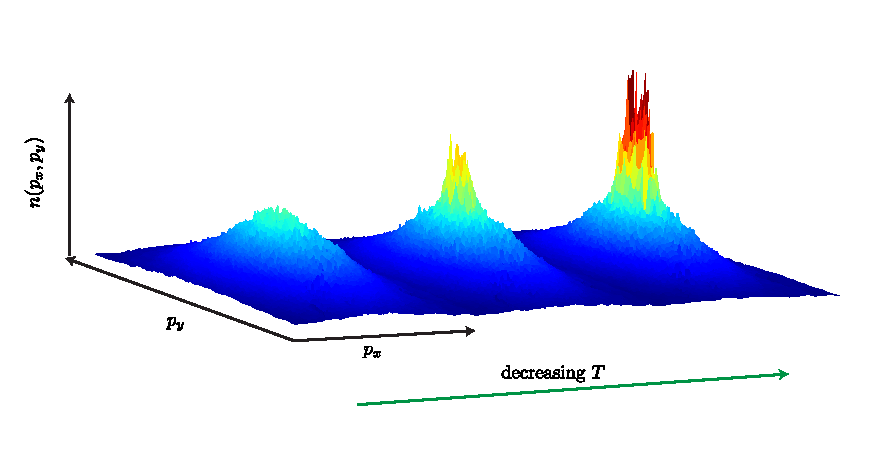
\includegraphics[]{Figures/Chapter2/BEC_transition.pdf}
\caption[Momentum distribution of atoms near $T_c$]{Momentum distribution of atoms near $T_c$ after a $\unit[21]{ms}$ TOF. As the atoms are cooled below $T_c$ a sharp peak in the momentum distribution appears indicating condensation.} 
\label{fig:BEC_transition}
\end{center}
\end{figure}



% were when the condensate
% was confined.
% or by measuring the
% TOF radii via absorption imaging, back-propagate what the original radii were when the condensate
% was confined.
% %
% \begin{align}
% 	n(\r)&=n_0e^{-(\frac{x^2}{2\sigma_x^2}+\frac{y^2}{2\sigma_y^2}+\frac{z^2}{2\sigma_z^2})}\nonumber \\
% 	&= \frac{15N}{8\pi R_xR_yR_z},
% \end{align}
% %
% where $\sigma_i=\omega_i^{-1}\sqrt{k_BT/m}$. Using the equipartition theorem we find that the spatial extension of the cloud and the temperature are related by 
% %
% \begin{equation}
% 	T=\frac{m}{k_B}\sigma_i^2\omega_i^2
% \end{equation}

% \note{TODO: what is my chemical potential?}


% For a given trapping potential $U(\r)$, the density distribution of a thermal ensamble is
% \begin{equation}
% 	n(\r) = n_0 e^{-\frac{U(\r)}{k_BT}}.
% \end{equation}
% %
% The temperature $T$ can be derived from the density distribution. For a 3D harmonic trap

